\section{Revisão da literatura}

% A missão de \gls{rvdb} é o processo de fazer com que duas espaçonaves se encontrem \cite{merriamRendezvous} e façam o acoplamento mecânico \cite{merriamDocking}.
% O procedimento envolve o alinhamento e a sincronização de atitude das espaçonaves para que possam estar em uma distância suficientemente segura para que a ancoragem\fn{Alternativamente, conhecido como atracação.} \emph{(berthing)} ocorra \cite{merriamBerthing}.
A missão de \gls{rvdb} é um conjunto de técnicas/procedimentos que viabilizam encontros orbitais e conexões seguras entre veículos espaciais, seja por acoplamento autônomo ou assistidos via astronautas ou centros de controles baseados em solo (docking) ou captura via manipuladores robóticos (berthing), também autônomos ou assistidos.
A operação de \gls{rvdb} se justificam pois existe a necessidade de executar tarefas como a montagem em órbita de unidades maiores, a ida do ônibus espacial \emph{(Space Shuttle)} para realizar a entrega de suprimentos na Estação Espacial Internacional (\gls{iss}) ou até mesmo para realizar o reparo de espaçonaves em órbita \cite{fehse2003}.
Portanto, é um tipo de operação chave para a prestação de serviços em órbita, conhecidos como \gls{oos}.

%%%%%%%%%  
% \subsection{Pioneirismo}

% O primeiro \gls{rvdb} entre duas espaçonaves ocorreu em 1966 \cite{nasa1stDocking}, quando Neil Armstrong e Dave Scott realizaram, de forma manual a aproximação (\emph{rendezvous}) na espaçonave \emph{Gemini} e acoplaram no veículo não-tripulado \emph{Agena}.
% No ano seguinte, ocorreu o primeiro \gls{rvdb} automático; as espaçonaves soviéticas \emph{Kosmos} 186 e 188 realizaram o acoplamento \emph{(docking)} entre si sem intervenção humana \cite{nasaAutmaticDocking1967}.
% Desde então, o conhecimento e a experiência obtidos com as missões Gemini e Apollo (1968-1972) foram posteriormente aplicadas com sucesso nas missões da Skylab (1973-1974) e \emph{Apollo--Soyuz} \cite{goodman2011rendezvous}.

% Durante a década de 1980, na Europa Ocidental, a tecnologia de \gls{rvdb} foi desenvolvida pela \gls{esa}.
% Inicialmente, essa técnica foi implementada no projeto \gls{mtff}, planejado para acoplar-se à estação espacial americana \emph{Freedom} \cite{goelz1992MtffFreedom} e à espaçonave europeia \emph{Hermes} \cite{worldspaceflightMTFF}.
% Após o cancelamento dos projetos \gls{mtff} e \emph{Hermes}, o \gls{atv} tornou-se a principal contribuição européia para o programa da \gls{iss} \cite{ellwood2007ATV2ISS}. O \gls{atv} foi concebido para realizar tarefas de abastecimento e manutenção da ISS \cite{atvDLR}.

% \begin{figure}[ht]
%     \label{fig:pioneirismo_ATV}
% \centering
% 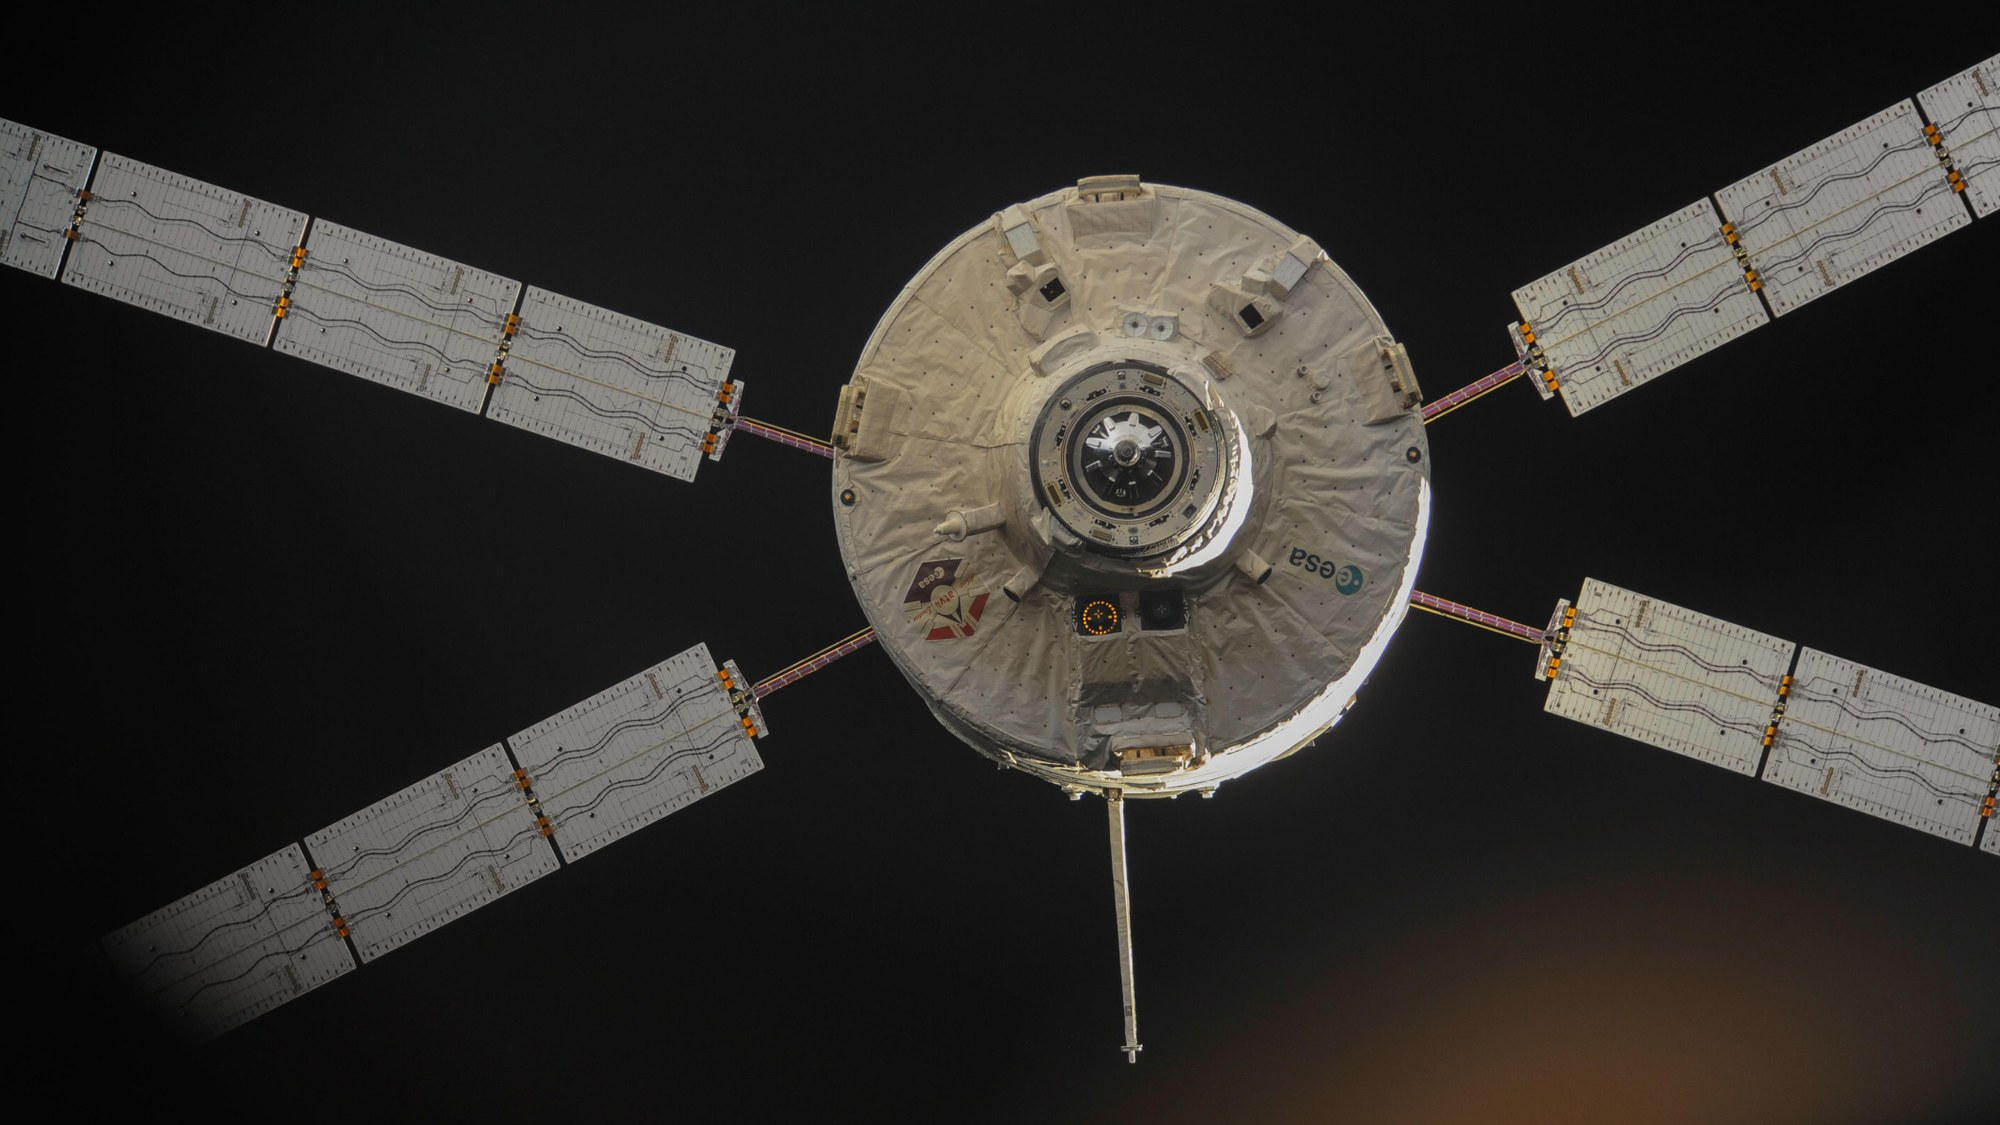
\includegraphics[width=1\linewidth]{1 Introducao/Imagens/2 Pioneirismo - ATV.jpeg}
% \caption{ATV (Automated Transfer Vehicle). Fonte: Deutsches Zentrum für Luft-und Raumfahrt (https://www.dlr.de/en/research-and-transfer/projects-and-missions/iss/europe-sets-a-course-for-the-iss).}
% \end{figure}

% Os veículos que realizaram \gls{rvdb} junto da ISS incluem o ônibus espacial dos \gls{eua}, a Soyuz russa e a espaçonave japonesa HTV \cite{nasaVisitingVehicles}.

\subsection{Pioneirismo}

Missões que envolvem \gls{rvdb} são justificadas por permitirem a montagem e expansão de estruturas orbitais, operações de manutenção em órbita e arquiteturas logísticas para exploração cislunar.
Como exemplos, a construção e operação da Estação Espacial Internacional (\emph{International Space Station, \gls{iss}}), dependeram de múltiplas operações de encontro e acoplamento para instalação dos módulos lançados separadamente \cite{nasaRVDBiss} e suportar reabastecimento de suprimentos regular.
De forma similar, as missões de serviço ao Telescópio Espacial Hubble evidenciaram a importância das operações de aproximação e acoplamento para reparos e modernizações em órbita \cite{hubbleRVDB}.
Por fim, requisitos de acoplamento e logística orbital associados ao \emph{Gateway} ajudam a justificar o papel de \gls{rvdb} como capacidade habilitadora em arquiteturas de exploração lunar \cite{gatewayRVDB}.

O primeiro \gls{rvdb} entre duas espaçonaves ocorreu em 1966 \cite{nasa1stDocking}, quando Neil Armstrong e David Scott realizaram manualmente a aproximação (\emph{rendezvous}) na espaçonave \emph{Gemini} e acoplaram ao veículo não tripulado \emph{Agena}.
No ano seguinte, ocorreu o primeiro \gls{rvdb} automático; as espaçonaves soviéticas \emph{Kosmos} 186 e 188 realizaram o acoplamento (\emph{docking}) sem intervenção humana \cite{nasaAutmaticDocking1967}.
Desde então, o conhecimento e a experiência obtidos com as missões Gemini e Apollo (1968--1972) foram posteriormente aplicados com sucesso nas missões da Skylab (1973--1974) e \emph{Apollo--Soyuz} \cite{goodman2011rendezvous}.

Durante a década de 1980, na Europa Ocidental, a tecnologia de \gls{rvdb} foi desenvolvida pela \gls{esa}.
Inicialmente, essa técnica foi implementada no projeto \gls{mtff}, planejado para acoplar-se à estação espacial americana \emph{Freedom} \cite{goelz1992MtffFreedom} e à espaçonave europeia \emph{Hermes} \cite{worldspaceflightMTFF}.
Após o cancelamento dos projetos \gls{mtff} e \emph{Hermes}, o \gls{atv} tornou-se a principal contribuição europeia para o programa da \gls{iss} \cite{ellwood2007ATV2ISS}. O \gls{atv} foi concebido para realizar tarefas de abastecimento e manutenção da ISS \cite{atvDLR}.

\begin{figure}[ht]
\centering
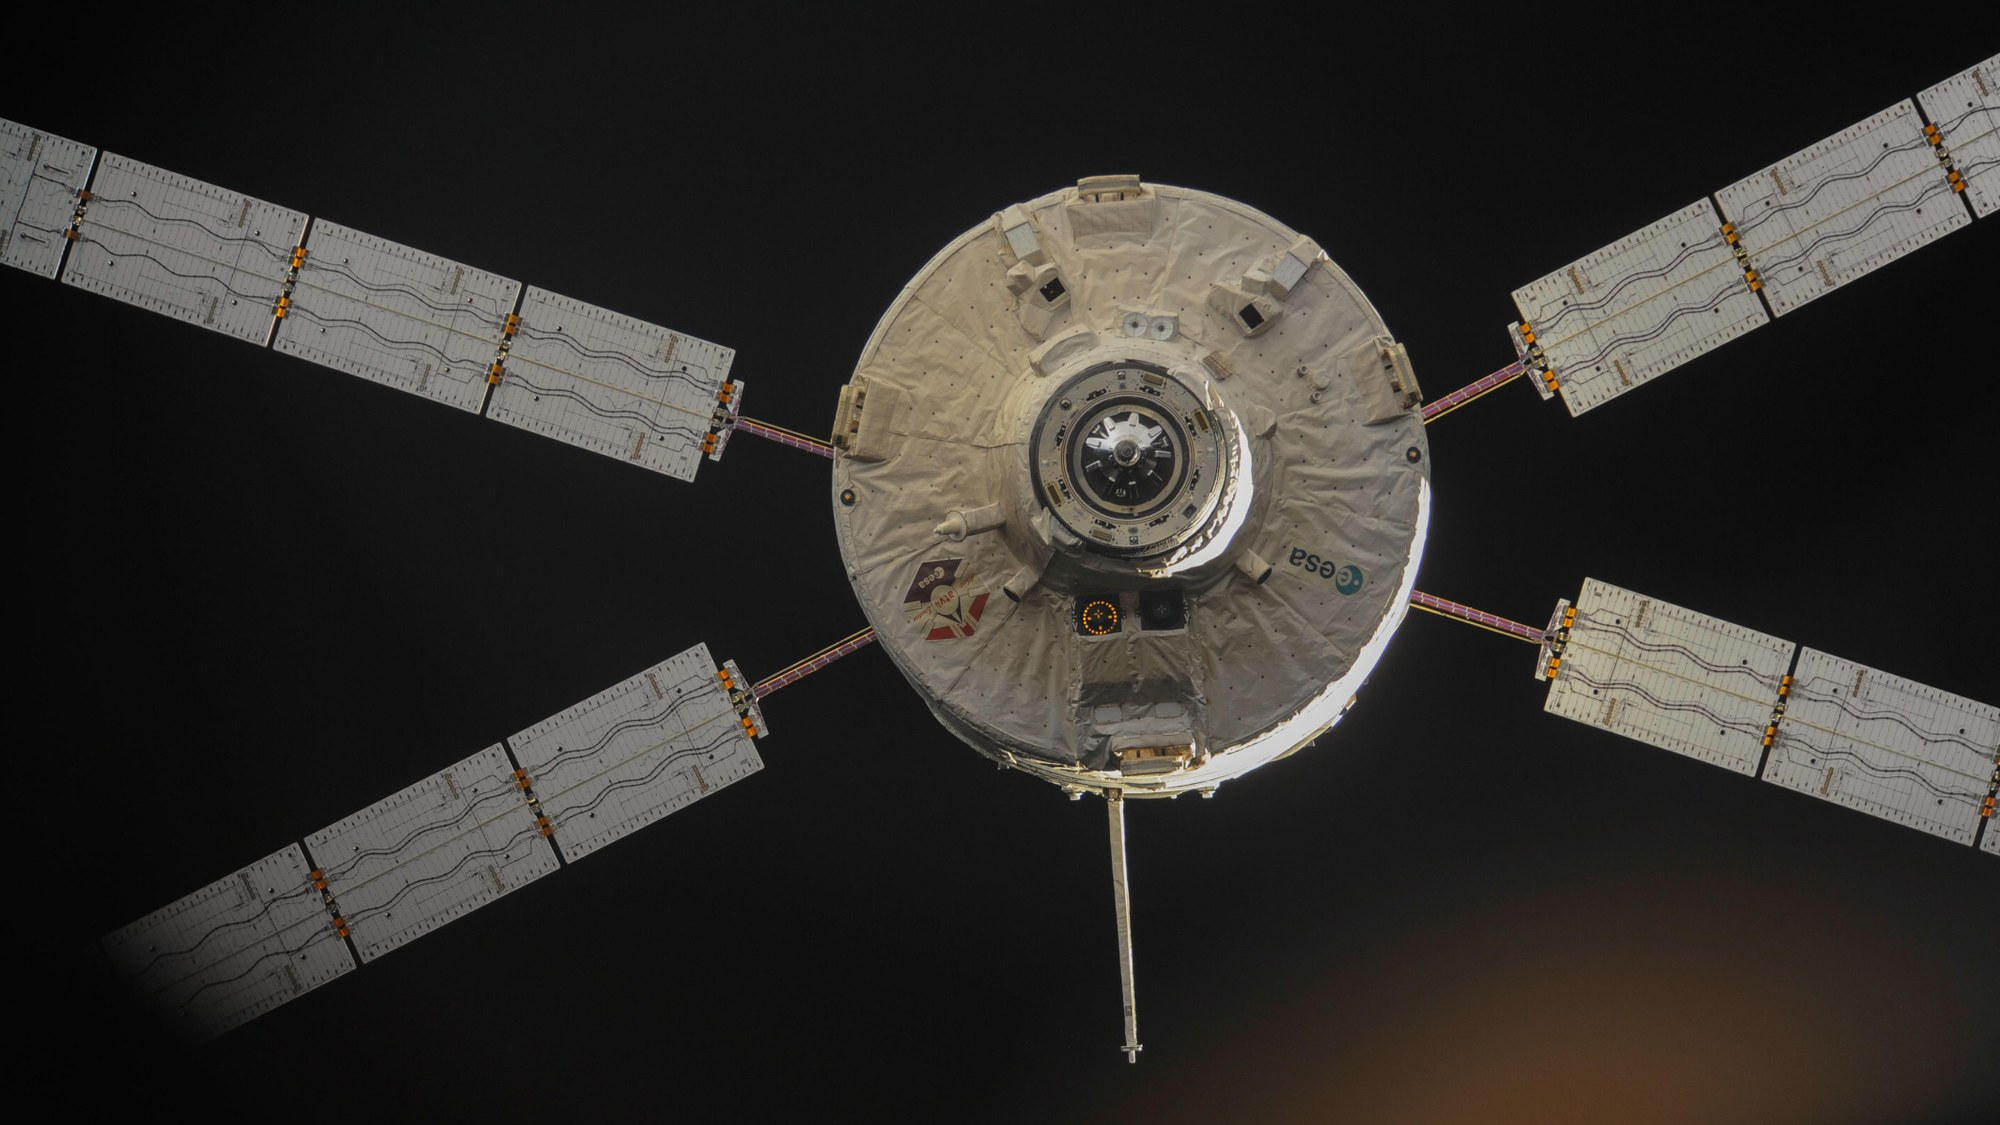
\includegraphics[width=1\linewidth]{1 Introducao/Imagens/2 Pioneirismo - ATV.jpeg}
\caption{ATV (Automated Transfer Vehicle). Fonte: Deutsches Zentrum für Luft- und Raumfahrt (DLR), disponível em \url{https://www.dlr.de/en/research-and-transfer/projects-and-missions/iss/europe-sets-a-course-for-the-iss}.}
\label{fig:pioneirismo_ATV}
\end{figure}

Os veículos que realizaram \gls{rvdb} junto da ISS incluem o ônibus espacial dos \gls{eua}, a Soyuz russa e a espaçonave japonesa HTV \cite{nasaVisitingVehicles}.


%%%%%%%%%%%%%%%%%%%%%%%%%%%%%%%%%%%%%%%%%%%%%%%%%%%%
% \section{Processo da missão de RVD/B}

% A missão de RVD/B pode ser dividida em fases, incluindo o lançamento, faseamento, aproximação de curta distância, aproximação final e acoplamento.
% A fase de lançamento é executada através de um veículo lançador, que também pode ser considerado no conceito geral do processo e por sua vez, a aproximação de curta distância pode ser dividida em fase de \emph{homing} e fase de \emph{closing} \cite{rvdProcesso}.

% \subsection{RVD/B pelo eixo radial (R-bar)}

% \begin{figure}[ht]
%     \label{fig:aproximacao_rbar_pioneirismo}
% \centering
% 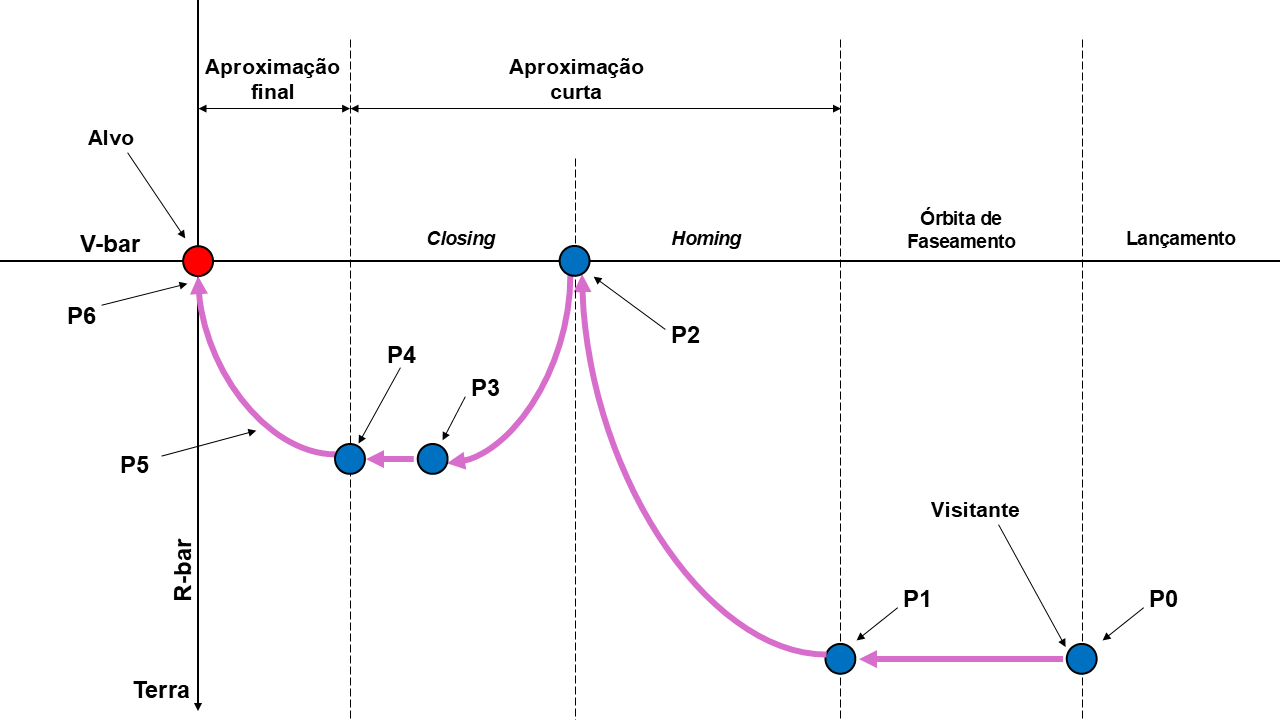
\includegraphics[width=1\linewidth]{1 Introducao/Imagens/2 Pioneirismo - RVDB R-bar.png}
% \caption{Aproximação do tipo R-bar. Fonte: Adaptado de \cite{fehse2003}.}
% \end{figure}

% Após a fase de lançamento, o veículo lançador insere a espaçonave visitante na órbita de injeção $\mathbf{(P0)}$.
% Durante a órbita de faseamento (\emph{phasing phase}), o veículo visitante realiza manobras sob o guiamento e comando realizados pela estação terrena para que os sensores de navegação do visitante possam obter os dados do veículo alvo.
% O objetivo dessa fase é ajustar o ângulo de fase orbital entre as duas espaçonaves, reduzindo a diferença dos planos orbitais $\mathbf{(P1)}$ e elevar o raio orbital para se igualar com o raio orbital do alvo $\mathbf{(P2)}$.
% Durante a \emph{homing phase}, o visitante se torna autônomo e seu objetivo é ir até o ponto $\mathbf{(P3)}$, o qual está localizado a alguns kilometros de distância do alvo. Essa fase possui o intuito reduzir tanto a velocidade relativa como a distância relativa.
% Na sequência, durante a \emph{closing phase}, o visitante reduz sua distância relativa ainda mais.
% A fase de aproximação final inicia a partir do ponto $\mathbf{(P4)}$, quando o visitante se aproxima do alvo pelo eixo radial \emph{(R-bar)} $\mathbf{(P5)}$ e finaliza quando o visitante encosta no alvo $\mathbf{(P6)}$.

% \subsection{RVD/B pelo vetor velocidade (V-bar)}

% A proximação pelo \emph{V-bar} se assemelha com a estratégia anterior; a diferença se dá a partir da fase de \emph{homing}.
% Na fase de \emph{closing}, o visitante realiza nova transferência de órbita $\mathbf{(P3)}$, dessa vez em um raio orbital menor quando comparado ao raio orbital do alvo, para que possa acelerar e se aproximar mais rapidamente do alvo.
% No início da aproximação final $\mathbf{(P4)}$, o visitante se aproxima em uma linha reta, de forma lenta e gradual até realizar o acoplamento mecânico com o alvo $\mathbf{(P5)}$.

% \begin{figure}[ht]
%     \label{fig:aproximacao_vbar_pioneirismo}
% \centering
% 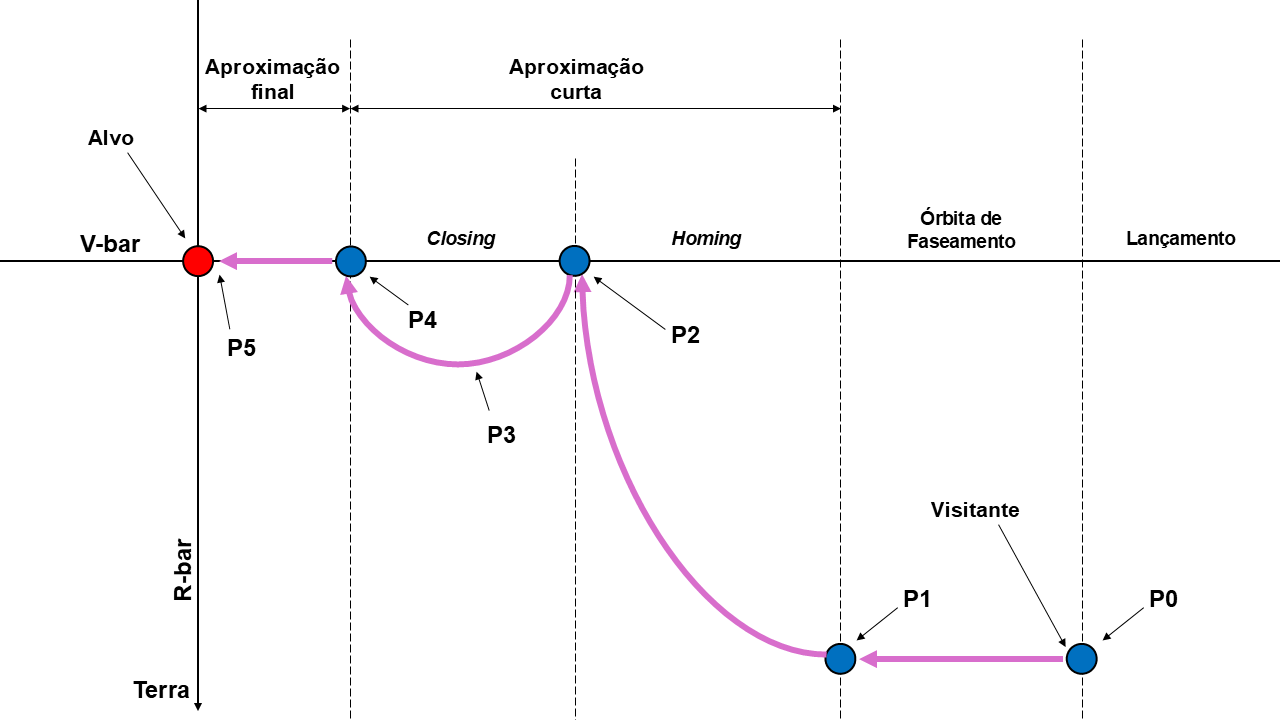
\includegraphics[width=1\linewidth]{1 Introducao/Imagens/2 Pioneirismo - RVDB V-bar.png}
% \caption{Aproximação do tipo V-bar. Fonte: Adaptado de \cite{fehse2003}.}
% \end{figure}
%%%%%%%%%%%%%%%%%%%%%%%%%%%%%%%%%%%%%%%%%%%%%%%%%%%%%%%%%
\section{Programa espacial Apollo}

O programa Apollo (1961--1972) consolidou capacidades operacionais diretamente relevantes para \gls{rvdb}, em especial na condução de fases de aproximação e acoplamento que exigem navegação orbital relativa, guiamento e tomada de decisão em tempo real \cite{RVDBapollo}.
Nesse contexto, a interação homem--máquina evoluiu de comandos diretos para um papel de supervisão, principalmente no monitoramento de estados, seleção de modos e gerenciamento de contingências, o que reduziu a dependência contínua da estação terrestre \cite{nevins1971}.

Como descrito por \cite{nevins1971}, requisitos associados a essa autonomia operacional incluíam:
\begin{enumerate}[label=(\roman*)]
    \item o sistema deveria ser capaz de completar a missão sem auxílio da estação terrestre;
    \item o sistema empregaria a participação humana sempre que isso pudesse simplificar ou melhorar a operação em comparação às sequências pré-estabelecidas das funções exigidas;
    \item o sistema deveria fornecer interfaces adequadas ao piloto por meio das telas e dos métodos de controle do sistema de orientação;
    \item o sistema deveria ser projetado de modo que as tarefas pudessem ser executadas por apenas um operador, de forma segura, permitindo o retorno seguro à Terra a partir de qualquer ponto da missão.
\end{enumerate}

Em operações de \gls{rvdb}, esses requisitos se traduzem na necessidade de (i) interpretar informações de navegação e orientação, (ii) intervir quando necessário em decisões de guiamento e controle e (iii) garantir continuidade operacional por meio de modos redundantes e transições seguras entre sistemas primários e de \emph{backup} \cite{nevins1971}.

